\documentclass[class=report,crop=false, 12pt]{standalone}
\usepackage[screen]{../myscratch}

\begin{document}


\titre[E]{Si ... alors ... sinon ...}
%===============================


\begin{enigme}[La suite de Syracuse]

La suite de Syracuse est une suite mystérieuse.
On part d'un nombre entier $x$, puis on applique un certain nombre de fois les instructions suivantes :
\begin{itemize}
  \item Si $x$ est pair, alors $x$ devient $x/2$ ;
  \item sinon, $x$ devient $3\times x + 1$.
\end{itemize}


\bigskip

Voici comment tester si un nombre $x$ est pair :
\begin{center}
\booloperator{\ovaloperator{\ovalvariable{x} modulo \ovalnum{2}} = \ovalnum{0}}
\end{center}

\textbf{Question.} En partant de $x=2017$, effectue $50$ fois l'opération. Combien vaut alors $x$ ?

\emph{Indication.} Après la première opération, on a $x=6052$, après la deuxième opération $x=3026$\ldots

\bigskip

%\begin{solution}
%Réponse : $184$.
%\end{solution}

\end{enigme}



\begin{enigme}

Scratch a un comportement bizarre !

\begin{itemize}
  \item Scratch part de la position $x=-150$, $y=+10$.
  
  \item Chaque jour on ajoute $10$ à $x$.
  
  \item Chaque jour on change aussi $y$ :
  \begin{itemize}
    \item Si $y<50$, alors $y$ devient $3 \times y$,
    \item sinon $y$ devient $y - 37$.
  \end{itemize}
  
\end{itemize}


\begin{center}
  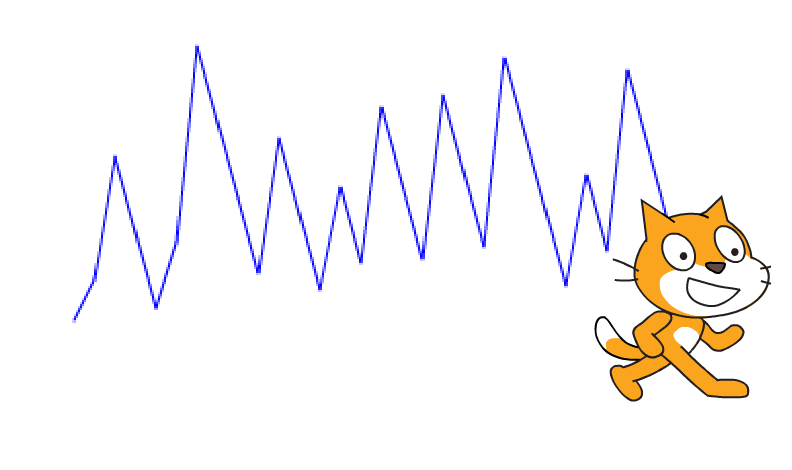
\includegraphics[width=0.6\textwidth]{ecran-07-eg2} 
\end{center}




\bigskip

\textbf{Question.} Au bout de $30$ jours, l'abscisse de la position de Scratch est $x=150$.
Combien vaut l'ordonnée $y$ ?

\bigskip


%\begin{solution}
%$y = 21$.
%\end{solution}

\end{enigme}



\begin{enigme}

Scratch part de la position $x=0$ et $y=0$, puis se déplace selon les instructions suivantes :
\begin{itemize}
  \item Si $x < 100$, on ajoute $7$ à $x$, sinon on retire $37$ à $x$.

  \item Si $y<100$, on ajoute $14$ à $y$, sinon on retire $22$ à $y$.
\end{itemize}

À chaque déplacement, il y a donc un mouvement horizontal puis un mouvement vertical.

\bigskip
%\sauteligne

Sur l'image ci-dessous, les $30$ premiers déplacements sont dessinés.
\begin{center}
  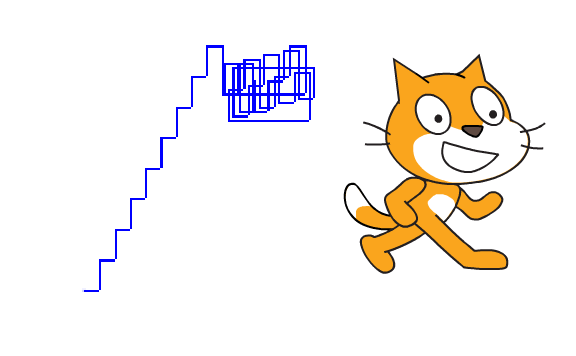
\includegraphics[width=0.6\textwidth]{ecran-07-eg3-new} 
\end{center}


\textbf{Question.}  Après $40$ déplacements, Scratch se retrouve en un point d'ordonnée $y=92$. Combien vaut alors l'abscisse $x$ ?

\bigskip



%\begin{solution}
%$x = 104$, $y = 92$, réponse attendue : $104$.
%\end{solution}

\end{enigme}

%\begin{enigme} % PAS STABLE
%
%Scratch se déplace. S'il touche une ligne horizontale bleue il avance, sinon il recule. S'il touche une ligne verticale rouge, il monte, sinon il descend.
%
%\begin{center}
%  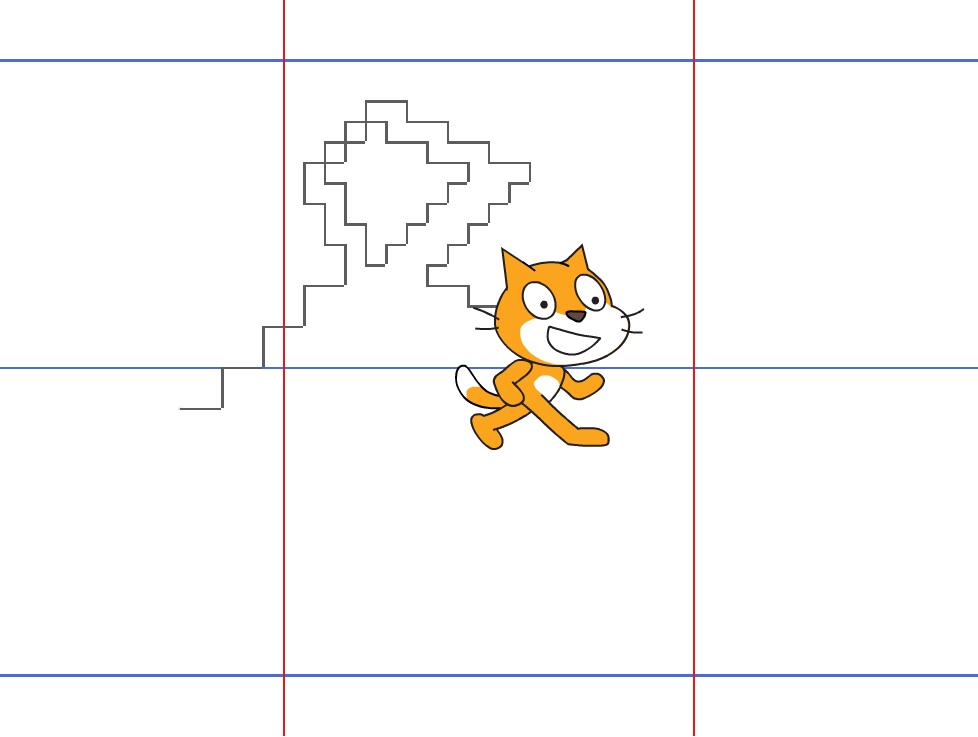
\includegraphics[scale=\scaleecran]{ecran-07-eg3} 
%\end{center}
%
%
%
%
%\textbf{Quadrillage.}
%Trace trois lignes horizontales en bleu qui traversent l'écran :
%une avec $y=-150$, une avec $y=0$, une avec $y=150$.
%Trace deux lignes verticales en rouge : une avec $x=-100$, une avec $x=100$.
%
%
%\bigskip
%\textbf{Déplacements}.
%Le lutin est le chat habituel.
%
%On commence d'abord par tester si le chat touche une ligne horizontale bleue.
%\begin{itemize}
%  \item Si c'est le cas, on ajoute $20$ à $x$,
%  \item sinon, on retire $10$ à $x$.
%\end{itemize}
%
%On teste ensuite, si le chat touche une ligne verticale rouge.
%\begin{itemize}
%  \item Si c'est le cas, on ajoute $20$ à $y$,
%  \item sinon, on retire $10$ à $y$.
%\end{itemize}
%
%
%À chaque déplacement il y a donc un mouvement horizontal, puis un mouvement vertical.
%
%
%
%\bigskip
%
%\textbf{Question.} Scratch part de $x=-150$ et $y=-20$. Après $40$ déplacements, il se retrouve en un point où $y=120$. Combien vaut alors $x$ ?
%
%\bigskip
%
%\emph{Indication.} Sur l'image ci-dessus, les $30$ premiers déplacements sont dessinés.
%
%
%%\begin{solution}
%%$x = 170$, $y = 120$, réponse attendue : $170$.
%%\end{solution}
%
%\end{enigme}

\end{document}

